\section{System Overview}
\begin{paracol}
    {2}

   The setup consists of a mobile manipulator (MIRTE Master) tasked with autonomously exploring an indoor laboratory environment, identifying and localizing objects, distinguishing between electronics and other objects and sorting these objects accordingly.

    The main task of the robot can be broken down into sub-tasks, these then fit into specific niches of the entire system architecture:
    \begin{enumerate}
    \item \textbf{Motion planning}
    \item \textbf{Perception}
    \item \textbf{Navigation}
    \end{enumerate}
    Figure \ref{tasks} showcases this idea.

    \begin{figure}[!htbp]
    \centering
    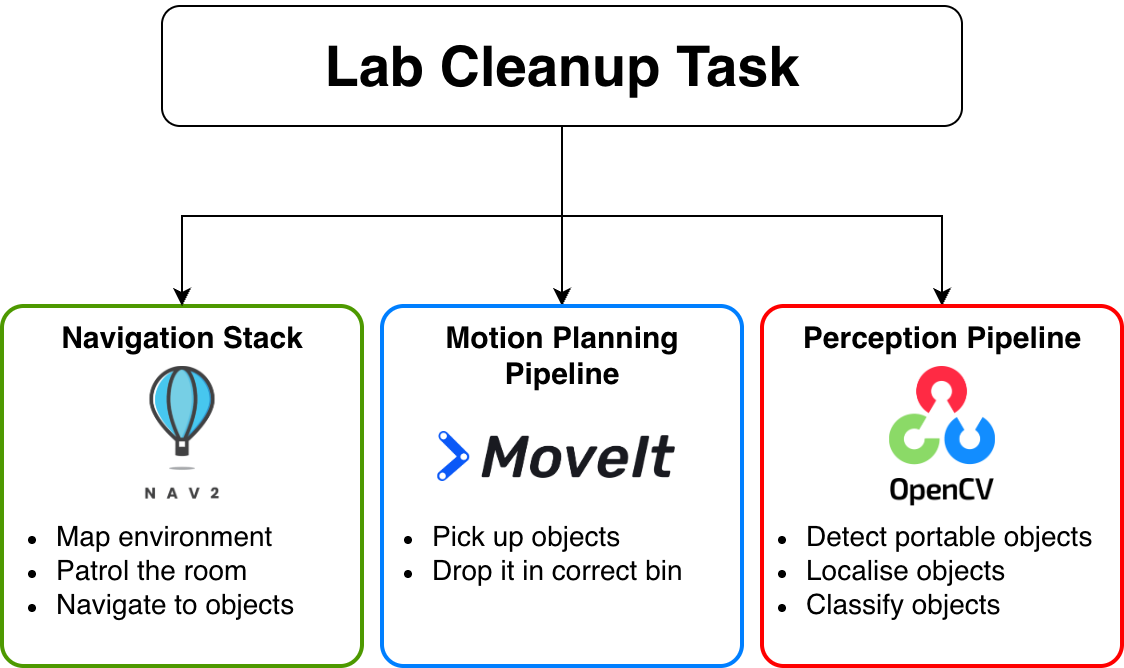
\includegraphics[width=1.02\linewidth]{latex/figures/Lab_Cleanup-Task Bins-4.drawio.png}
    \caption{Three main tasks of the Robot}
    \label{tasks}
    \end{figure}

    The scope of this project includes how different mapping, navigation and perception approaches influence the performance of the whole system. The highest performing combination of approaches is then chosen for use in the respective subsystems.
    
    %\medskip
    %\centerline{\rule{7.8cm}{0.4pt}}
    \subsection{System Architecture}
    
    The system level strategy consists of how the robot behaves in each scenario that it will find itself. The tasks described above are used as a guideline to construct the full system level strategy. The standard in robotics for such navigation and perception heavy tasks is to use a global behavior tree that describes how the robot ought to behave in certain situations. This system level architecture as shown in Figure~\ref{fig:tree} is also used here to describe and execute the cleaning strategy.
    \syncallcounters
    \switchcolumn
    \begin{figure}[H]
        \centering
        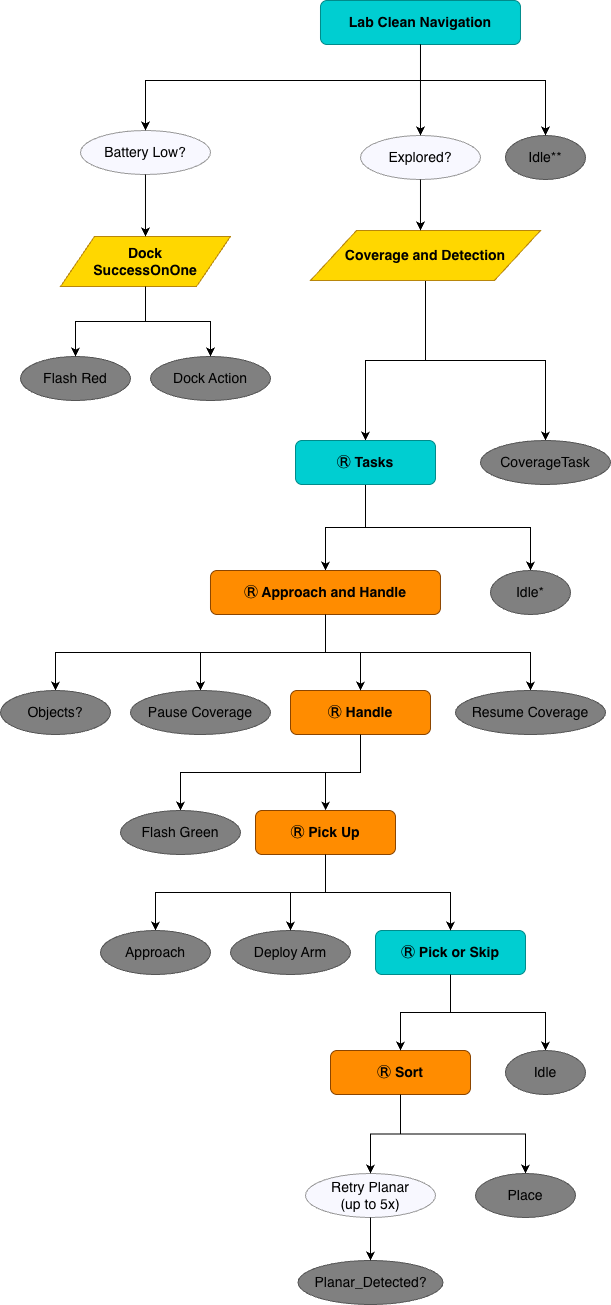
\includegraphics[width=1.01\linewidth]{latex/figures/labclean_tree.drawio-simple tree.drawio (1).png}
        \caption{Behaviour Tree}
        \label{fig:tree}
    \end{figure}
    The behavior tree provides a hierarchical approach for coordinating navigation, perception and cleaning actions, cascades through the modules. It also can easily be visualised, simplifying debugging significantly. As can be seen from the tree, the robot will initially drive around. When it detects an object, it will approach, pick it up and place it in the correct basket.
    \syncallcounters
    \end{paracol}
    \newpage
    \begin{paracol}
        {2}
    \subsection{Mechanical}
    
    The CAD-model of this rendition of the MIRTE Master can be found using this link: \href{https://cad.onshape.com/documents/ee158bec245e3fe46f63c9ce/w/a0c8c76ba94ff339073118d4/e/a16fbc4a88cf67fd9fba6368?renderMode=0&uiState=6a2aaef65092a9418fe6a8f1}{CAD-Model}.
    \medskip
    \centerline{\rule{7.8cm}{0.4pt}}

    \subsubsection{Original MIRTE Master Platform}

    The project is based on the MIRTE Master V2. The platform consists of a mobile base propelled by four individually driven mecanum wheels and a robotic arm, allowing the robot to navigate through an environment and interact with objects.

    The original MIRTE Master hardware consists of three main parts:
    \begin{enumerate}
    \item \textbf{Mobile base}
    \item \textbf{Electronics}
    \item \textbf{Robotic arm}
    \end{enumerate}
    The mobile base utilizes four geared DC motors with Hall encoders, connected to 97 mm mecanum wheels. This allows the robot to move in multiple directions without having to turn first, which is useful for navigating in small indoor spaces. The base also contains various sensors, such as rearward facing ultrasonic sensors, an IMU, a 2D LiDAR and an RGBD (depth) camera mounted on the robotic arm.

    The electronics of the original platform are based on an Orange Pi 3B and a Raspberry Pi Pico H. The Orange Pi functions as the main computer, while the Pico is used for lower-level control tasks such as controlling the motors and general interfacing. The MIRTE Master also includes a custom-made PCB to connect the motors, sensors, and power system in a structured manner. The main power source for the MIRTE Master is a 5Ah 12V Lion Parkside drill battery. No significant changes were made to the electronics used for this project.
    
    The robotic arm is mounted on top of the mobile base and has four degrees of freedom, which are driven by four serial bus servo motors of varying strengths. A gripper and RGBD camera are mounted at the end of of the arm for object scanning and manipulation.
    
    \medskip
    \centerline{\rule{7.8cm}{0.4pt}}

    \subsubsection{Hardware Components}

    The most important original hardware components can be seen in \href{https://matt-rbt.github.io/Lab-Cleanup-Robot-using-the-Mirte-Master-Platform/materials/}{Materials}.
    \syncallcounters
    \switchcolumn
    These components provide a useful base platform for a mobile manipulation task. However, for this project, the original configuration needed some changes. The robot had to be adapted for a laboratory-cleanup task, where it should be able to move around in a laboratory environment, detect waste on the floor, and eventually collect and move objects into bins.

    \subsubsection{Design Goals for the Modified Robot}

    The goal of the hardware modifications was to make the MIRTE Master more suitable for collecting and transporting small waste objects. This required changes to the chassis and and gripper design.
    
    The main design goals were:
    \begin{itemize}
    \item Add space for collecting and separating waste.
    \item Mount the camera in a useful position for object recognition.
    \item Improve the battery mounting system.
    \item Improve cable management.
    \item Modify the gripper so it can pick up waste objects more reliably.
    \end{itemize}
    \medskip
    \centerline{\rule{7.8cm}{0.4pt}}

    \subsubsection{Chassis Modifications}
    
    The original MIRTE Master chassis was designed as a general-purpose mobile manipulator base. For this use case, the robot also needed to carry waste bins and support the manipulator during picking tasks. Therefore, the chassis was modified to improve strength and usability.
    
    The chassis consists of six side panels and a top and a bottom plate. In the original model, the top and bottom plates were made out of clear PMMA. While PMMA allows the user to see the status of the electronics clearly by looking at the LEDs on the inside, it also has a tendency to shatter easily if bent too much. During early testing of the MIRTE Master it has already shown that the PMMA was not a good choice for any type of loading resulting in shattered PMMA. Therefore a change to the material of all plates from PMMA to aluminium with a similar stiffness was essential, the difference of this being that aluminium can bend more without shattering. To still be able to see the status of the electronics by the LEDs, the six side panel elements were 3D-printed using a slightly translucent material.
    
    Two separate waste bins were added to the robot. These bins allow the robot to collect, store and separate objects after picking them up.
    \syncallcounters
    \end{paracol}
    \newpage
    \begin{paracol}
        {2}
    \subsubsection{Gripper Modifications}
    
    The gripper is an important part of the laboratory-cleanup robot because it directly interacts with the objects that need to be collected. The original MIRTE Master gripper is useful as a general robotic gripper, but the cleanup task requires it to handle different small objects reliably.

    The original gripper geometry is suitable for holding small and large objects, however, the gripping surface is not. Electronic trash tends to have small contact points for the gripper, so good gripping performance is a must-have. For improving the grip on objects, the contact patches are layered with a layer of soft 83A TPE, coated with an additional layer of Bison Rubber anti-slip coating.
    
    During the initial testing phase of the RGBD camera, it was found that the mounting location for it was too low to the ground for it to be able to confidently display any accurate results regarding the distance towards objects. While this was the intended way for the camera to be implemented, for this project it was a better plan to mount this RGBD camera onto the end of the arm, right above the gripper. This gives it elevation which makes it able to look slightly more downward and therefore it could more accurately display distances. This also makes the need for the secondary RGB camera mounted onto the gripper insignificant, as the RGBD camera can also be used for object detection.
    
    \medskip
    \centerline{\rule{7.8cm}{0.4pt}}

    \subsubsection{Current Design}
    The finalised design is available for viewing \href{https://matt-rbt.github.io/Lab-Cleanup-Robot-using-the-Mirte-Master-Platform/mechanical/}{here}.
    %\todo{Screenshot van de robot}
    %\begin{figure}
    %    \centering
    %    \includegraphics[width=0.5\linewidth]{}
    %    \caption{Caption}
    %    \label{fig:placeholder}
    %\end{figure}
    
    \medskip
    \centerline{\rule{7.8cm}{0.4pt}}

    \subsection{Navigation}

    The navigation stack of this robot is responsible for two main tasks:
    \begin{itemize}
    \item Mapping
    \item Coverage
    \end{itemize}
    \medskip
    \centerline{\rule{7.8cm}{0.4pt}}
    \subsubsection{Mapping}
    
    Before the robot can navigate properly through the environment and ensure proper coverage, this environment must first be known. That is where mapping approaches can be helpful. Several advanced and specialised mapping approaches already exist, but in this paper only one was considered: `frontier based mapping'. 
    \syncallcounters
    \switchcolumn
    Unlike less advanced alternatives, frontier based mapping allows the robot to start navigating the space and propagate its behavior further down the tree as soon as the environment is mapped sufficiently. Once the environment is mapped sufficiently, the robot is allowed to navigate the space and propagate its behavior further down the tree.
    \medskip
    \centerline{\rule{7.8cm}{0.4pt}}
    \subsubsection{Coverage Planning Algorithms}

    This section presents the algorithms employed for the discovery of portable objects. While a comprehensive technical analysis of these algorithms is beyond the scope of this work, they are described with sufficient detail to enable understanding of their application within our framework. For in-depth technical details and formal derivations, the reader is referred to the original publications cited herein.
    To demonstrate the different navigators, a costmap of the Pulse Breakout room is used. This map was obtained during testing of the coverage methods.
    Furthermore Nav2 \citep{macenski2020marathon2} is used for low level motion planning and execution aswell as realtime control and costmap generation.

    %In order to demonstrate the different navigators, a map provided by the \href{https://github.com/MartijnWisse/mirte\_navigation}{MIRTE Navigation} ROS2 package is used. \newline
    % . . . shows the costmap generated by Nav2.

\paragraph{Preprocessing}

    Before the map can be used to plan a path, a common preprocessing algorithm can be abstracted.
    Coverage path planners generally use either a binary map of the free space,
    (free=1, occupied=0) or the polygons constructed from the boundaries of the free space.

    The input to the algorithm can be any 2D image displaying the free and occupied pixels.
    In this case the input will be the costmap directly. First the costmap is thresholded to create a Figure~\ref{fig-costmap1}, which is the first output.

    \begin{figure}[H]
        \centering
        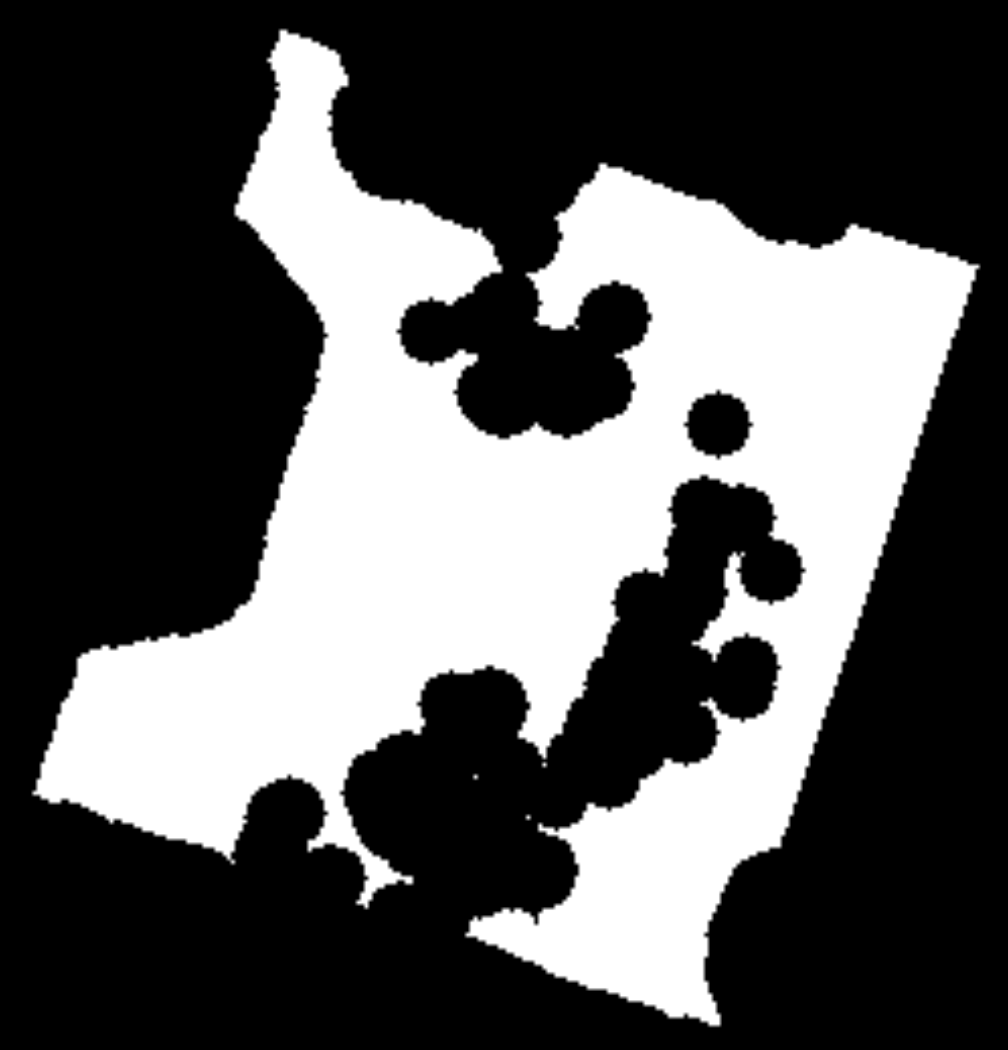
\includegraphics[width=0.8\linewidth]{latex/figures/Screenshot 2026-06-11 at 22.27.16.png}
        \caption{Binary costmap generated by thresholding the Nav2 costmap into free and occupied space.}
        \label{fig-costmap1}
    \end{figure}
    \syncallcounters
    \end{paracol}
    \newpage
    \begin{paracol}
        {2}
    Then, using this binary costmap, the contours in \ref{fig-map_contours__} are extracted.
    \begin{figure}[!htbp]
    \centering
    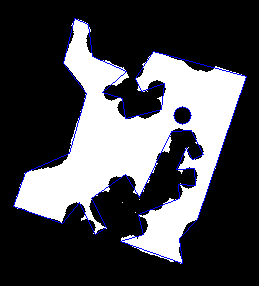
\includegraphics[width=0.7\linewidth]{content/figures/navigator_results/Detected_contours_(red).png}
    \caption{Contours extracted from the binary costmap representing the boundaries of free space.}
    \label{fig-map_contours__}
    \end{figure}

    \paragraph{Morphology-Based Skeleton Path Planner}

   The first implemented method, based on the work of \citep{skeleton}, \citep{skeleton2}, derives a coverage path from the morphological skeleton of the free space. The algorithm is visible in the Appendix.

    %fix een label voor dit aub
    
    The free space is extracted using the methods discussed in the previous section. The polygons are used and converted to a binary map as to not produce too many branches for the robot to navigate through. This map is then skeletonised to extract waypoints, see Figure~\ref{fig-skeleton_free__}.

    \begin{figure}[!htbp]
    \centering
    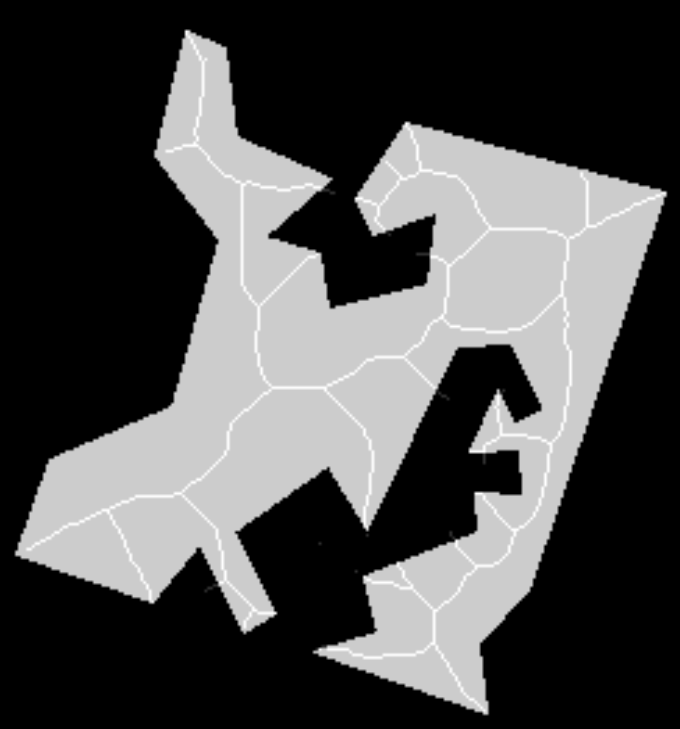
\includegraphics[width=0.7\linewidth]{latex/figures/Screenshot 2026-06-12 at 11.06.44.png}
    \caption[]{Morphological skeleton extracted from the free-space representation of the environment.}
    \label{fig-skeleton_free__}
    \end{figure}
    Once the waypoints are obtained, a graph is constructed and leaf nodes are extracted. In the graph leaf nodes are defined by there single connection to the rest of the skeleton, these are seen as endpoints of the path. Finally, starting from the closest leaf node to the robot, the full path is planned by recursively tracing the graph from the current leaf node to the nearest unvisited leaf node.

    \syncallcounters
    \switchcolumn

    \begin{figure}[!htbp]
    \centering
    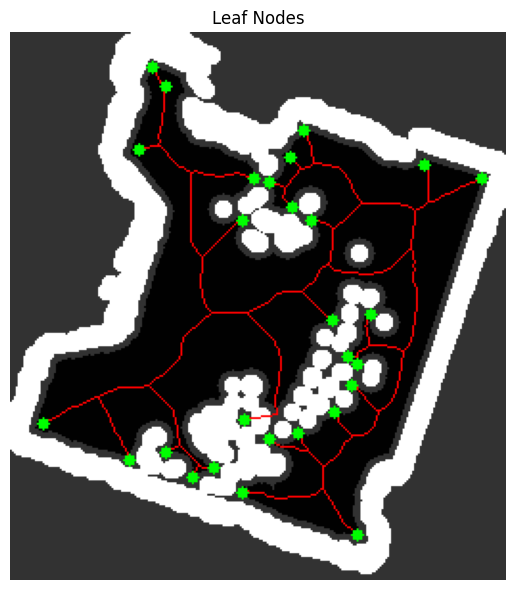
\includegraphics[width=0.99\linewidth]{content/figures/navigator_results/skeleton_tree_leaves.png}
    \caption{Leaf nodes identified on the skeleton graph, representing endpoints used during path generation.}
    \label{fig-skeleton_leaves__}
    \end{figure}
    
    Finally, starting from the closest leaf node to the robot, the full path is planned by recursively tracing the graph from the current leaf node to the nearest unvisited leaf node. This can be seen in Figure \ref{fig:full_path__}.

    \begin{figure}
        \centering
        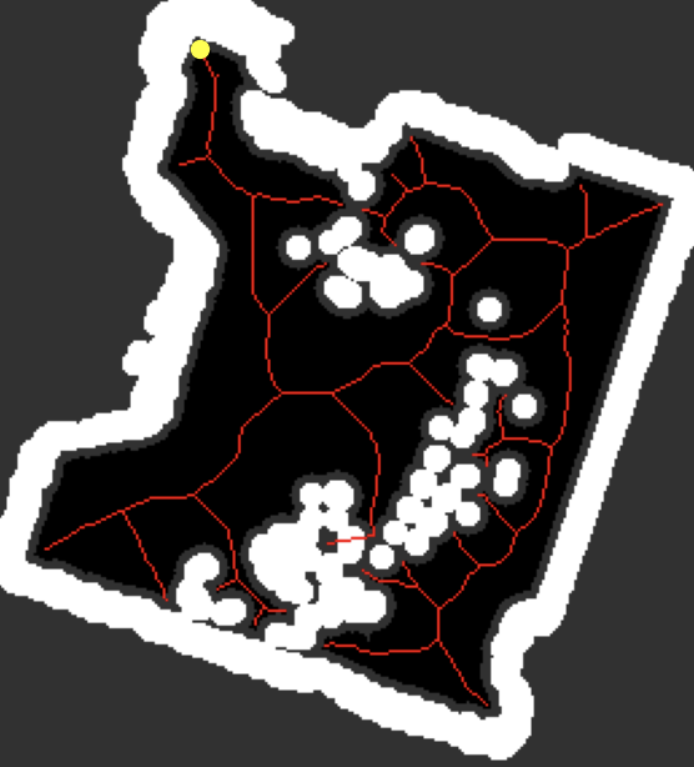
\includegraphics[width=0.7\linewidth]{latex/figures/Screenshot 2026-06-12 at 11.10.58.png}
        \caption{Fully planned path}
        \label{fig:full_path__}
    \end{figure}
    \syncallcounters
    \end{paracol}
    \newpage
    \begin{paracol}
        {2}
    \paragraph{Grid-Based Spanning Tree Planner}
    Secondly, a grid-based spanning tree algorithm is used to plan a full coverage path over the map. This planner is based on the work of \citep{SpanningTree2001}.

    As opposed to the Skeleton planner, this planner makes use of the binary costmap directly. Using this binary costmap, it is further discretised to a grid which is the fraction of the resolution of the original costmap, see Figure~\ref{fig-spanning_grid__}.

    \begin{figure}[!htbp]
    \centering
    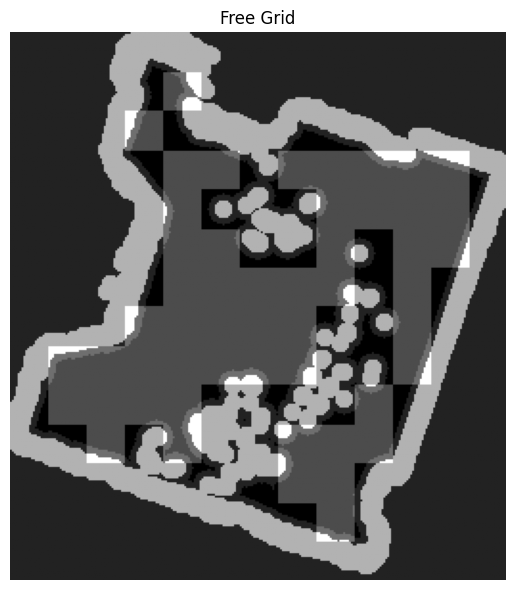
\includegraphics[width=0.7\linewidth]{content/figures/navigator_results/spanning_tree_grid.png}
    \caption[]{Downsampled free-space grid used to construct the spanning tree graph.}
    \label{fig-spanning_grid__}
    \end{figure}
    \syncallcounters

    A degree first search (DFS) is conducted over the free cells, from which sparse waypoints are created. This can be seen in Figure \ref{fig:fig-spanning_dfs__}.

    \begin{figure}
        \centering
        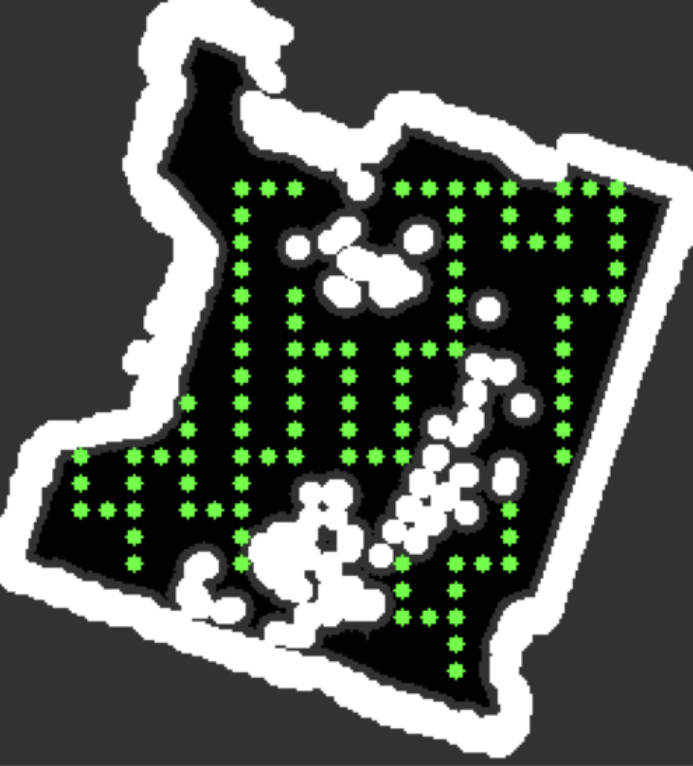
\includegraphics[width=0.7\linewidth]{latex/figures/Screenshot 2026-06-12 at 11.16.30.png}
        \caption{Depth-first search spanning tree generated over the free-space grid.}
        \label{fig:fig-spanning_dfs__}
    \end{figure}
    A black image, of the same resolution as the original costmap is then created and white squares, with half the cell width, are placed in the center of each cell and in between each cell. Waypoints are created from the contours of this tree. These waypoints represent a circumnavigation around the DFS tree.
    \syncallcounters
    \switchcolumn
    \begin{figure}[!htbp]
    \centering
    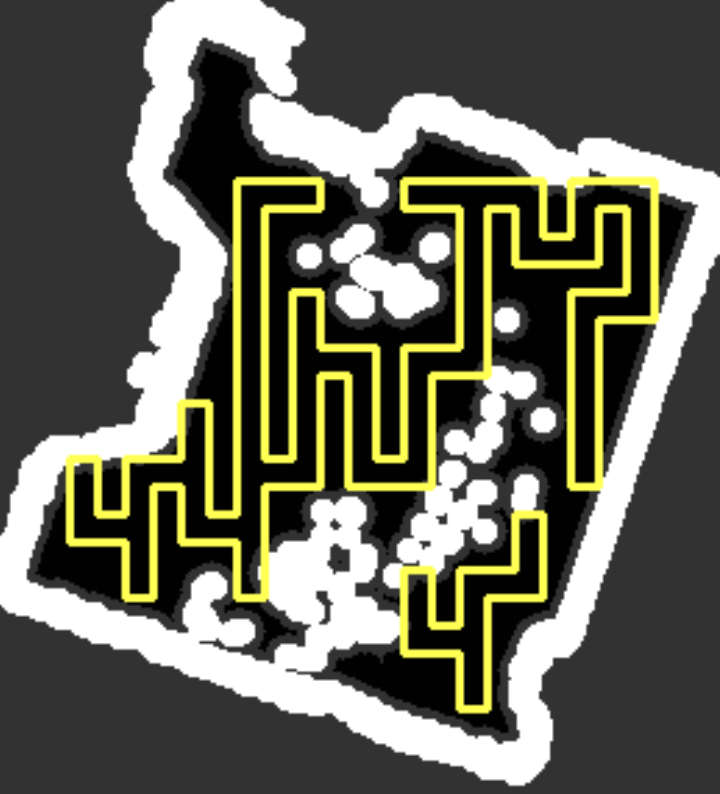
\includegraphics[width=0.7\linewidth]{latex/figures/Screenshot 2026-06-12 at 11.19.59.png}
    \caption[]{Coverage waypoints generated by tracing the contour around the spanning tree structure.}
    \label{fig-spanning_waypoints__}
    \end{figure}
    A segment from this circumnavigation is then removed from the path.

    \begin{figure}
        \centering
        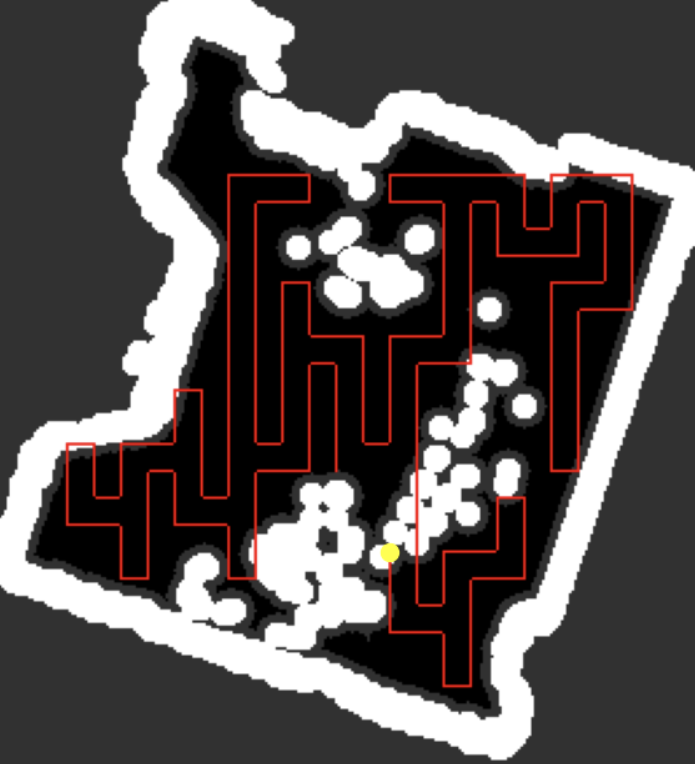
\includegraphics[width=0.7\linewidth]{latex/figures/Screenshot 2026-06-12 at 11.29.22.png}
        \caption{The path with circumnavigation removed.}
        \label{fig:placeholder}
    \end{figure}
    A lab cleanup robot must not blindly follow waypoints. If it does it might collide with obstacles near the map boundary or collide with moving objects. \newline
    Nav2 implements several low level real-time trajectory planners that plan inside the live updating costmap \citep{macenski2023survey}. They handle how the waypoints are followed and how much influence the map ought to have on the generated trajectory. The system described in this section implements an MPPI controller \citep{williams2017mppi} due to its superior performance in highly dynamic environments, like labs where students or people frequently walk \citep{elbouhy2024ros2planning}. Other planners that were considered include DWB (Dynamic Window Approach Behavior-based) \citep{thrun1997dwa} and RPP (Regulated Pure Pursuit) \citep{macenski2023regulated}.
    \end{paracol}
    \newpage
    \subsection{Perception}
    \begin{paracol}
        {2}
    Perception is responsible for object detection, classification and spatial localization. For this study the object detection and localization approaches were limited to two. A \textbf{2D detection and depth projection} approach and 3D segmentation with \textbf{point cloud clustering}.
    As for classification methods, this study evaluates a classical cv approach, as well as a classification model based approach.
    
    Originally, objects where categorised into:
    \begin{enumerate}
    \item Graspable vs non-graspable
    \item Electronics vs non-electronics
    \end{enumerate}
    However, due to the limitations of the hardware of the standard MIRTE Master package (relatively low-quality camera and limited computing power) the scope got reduced to:
    \begin{enumerate}
    \item Graspable vs non-graspable
    \item Colourful vs greyscale
    \end{enumerate}
    \subsubsection{Perception 2D}
    For determining the type, and possibly the distance of objects, a YOLO26 ('You Only Look Once-26') object classification model was used. A dataset was trained by recording videos using the USB Camera included in the MIRTE Master hardware package, of which one in every fifteen frames got extracted to use for the training dataset. A picture of four frames in different environments is shown below.
    \switchcolumn

    \begin{figure}[!htbp]
    \centering
    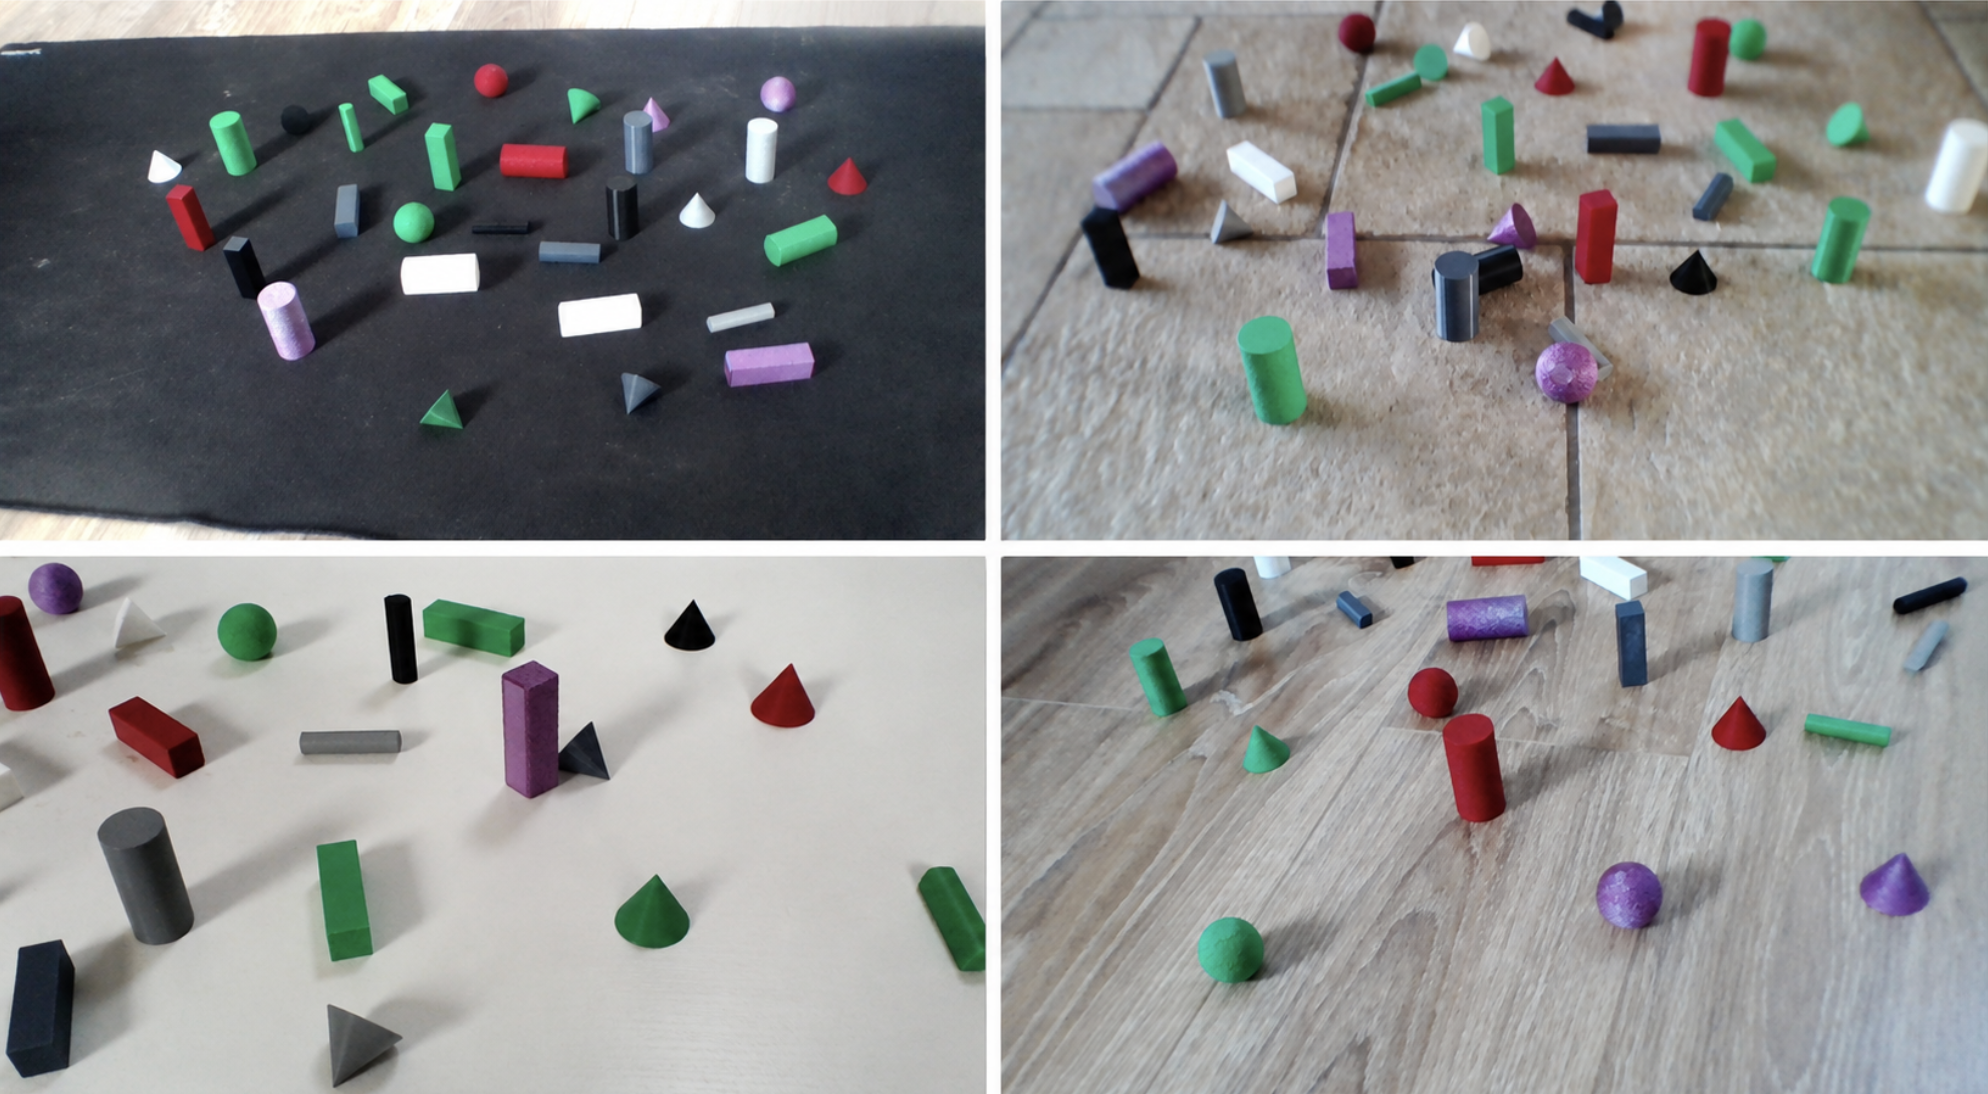
\includegraphics[width=0.99\linewidth]{latex/figures/Screenshot 2026-06-11 at 11.59.18.png}
    \caption[]{Picture of four individual frames}
    \label{fig_trainingdataset}
    \end{figure}
    
    \syncallcounters

    \paragraph{Why YOLO26 was used:}
    The YOLO object-detection family is well established, with YOLO26 being the most recent generation. YOLO26 was chosen because the robot has to detect and classify objects from a live camera on the MIRTE Master platform, which has limited processing power as it uses an OrangePi 3B which has limited computational capabilities. Object detection with limited processing power requires a lightweight model with fast inference times while still maintaining accuracy. YOLO26 is suitable for this because it was designed with deployment on low-power devices in mind. It changed the post-processing pipeline to NMS-free inference, simplified bounding-box predictions and supports deployment formats commonly used for low-power devices \citep{yolo26keyarchitecturalenhancements}.
   
    In this case, the RK3566 NPU of the OrangePi 3B can be used for improving the performance, reducing the total inference time \citep{Yolo11RK3566}. For this model, the Nano variant of YOLO26 was chosen to minimize inference times. Another benefit of the newer YOLO26 variant over the older variants is that YOLO26 allows for oriented bounding boxes. Unlike standard bounding boxes, oriented bounding boxes also estimate the rotation of recognised objects \citep{2026ultralyticsyoloevolutionoverview}. This could be useful for complex grasping tasks where orientation of the gripper is crucial. However, this project only uses standard object detection.

    \paragraph{Training:}
    Training was done manually using Label Studio. Initially, roughly 280 frames were captured in four different environments. Due to a large amount of blurring within the images, about 100 pictures were deleted. Of the remaining 180 pictures, 60 pictures were imported into Label Studio and labelled per colour: green, red, purple, white, light-grey, dark-grey and black. In total, 1206 bounding boxes were drawn. The relevant results of the training session are shown within the figure below.

    \end{paracol}
    \newpage
    \begin{paracol}
        {2}

    \begin{figure}[!htbp]
    \centering
    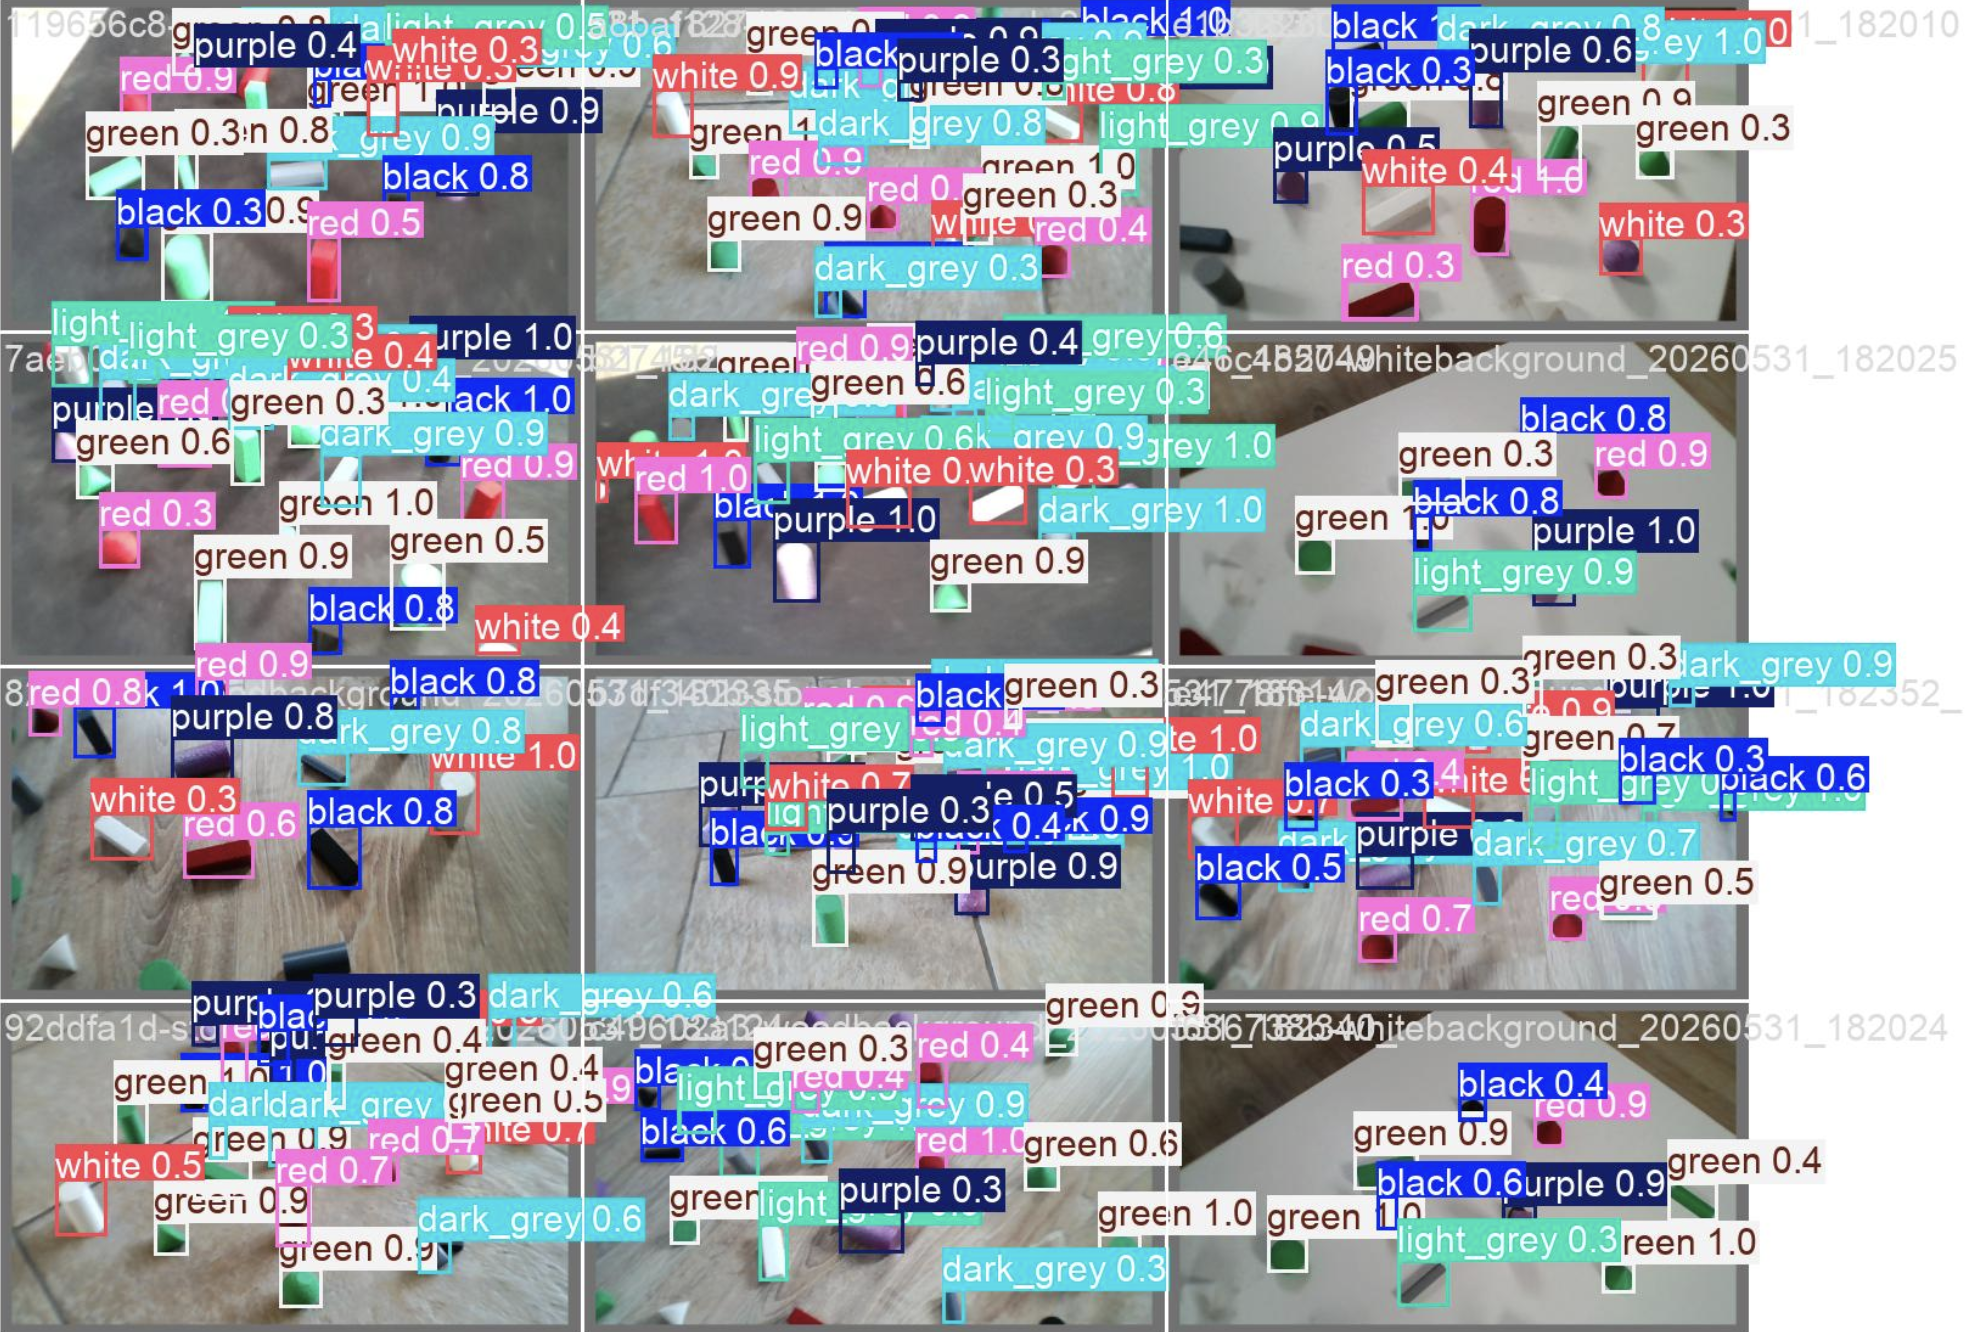
\includegraphics[width=0.99\linewidth]{latex/figures/Screenshot 2026-06-11 at 12.01.41.png}
    \caption[]{Figure of tests performed during training}
    \label{fig_trainingdatasetresults}
    \end{figure}
    %\smallskip
    \centerline{\rule{7.8cm}{0.4pt}}
    The curves in the figure below show that the model converged during trading. This means that the model actually learns while training instead of making random or unstable decisions.
    \syncallcounters
    
    \begin{figure}[!htbp]
    \centering
    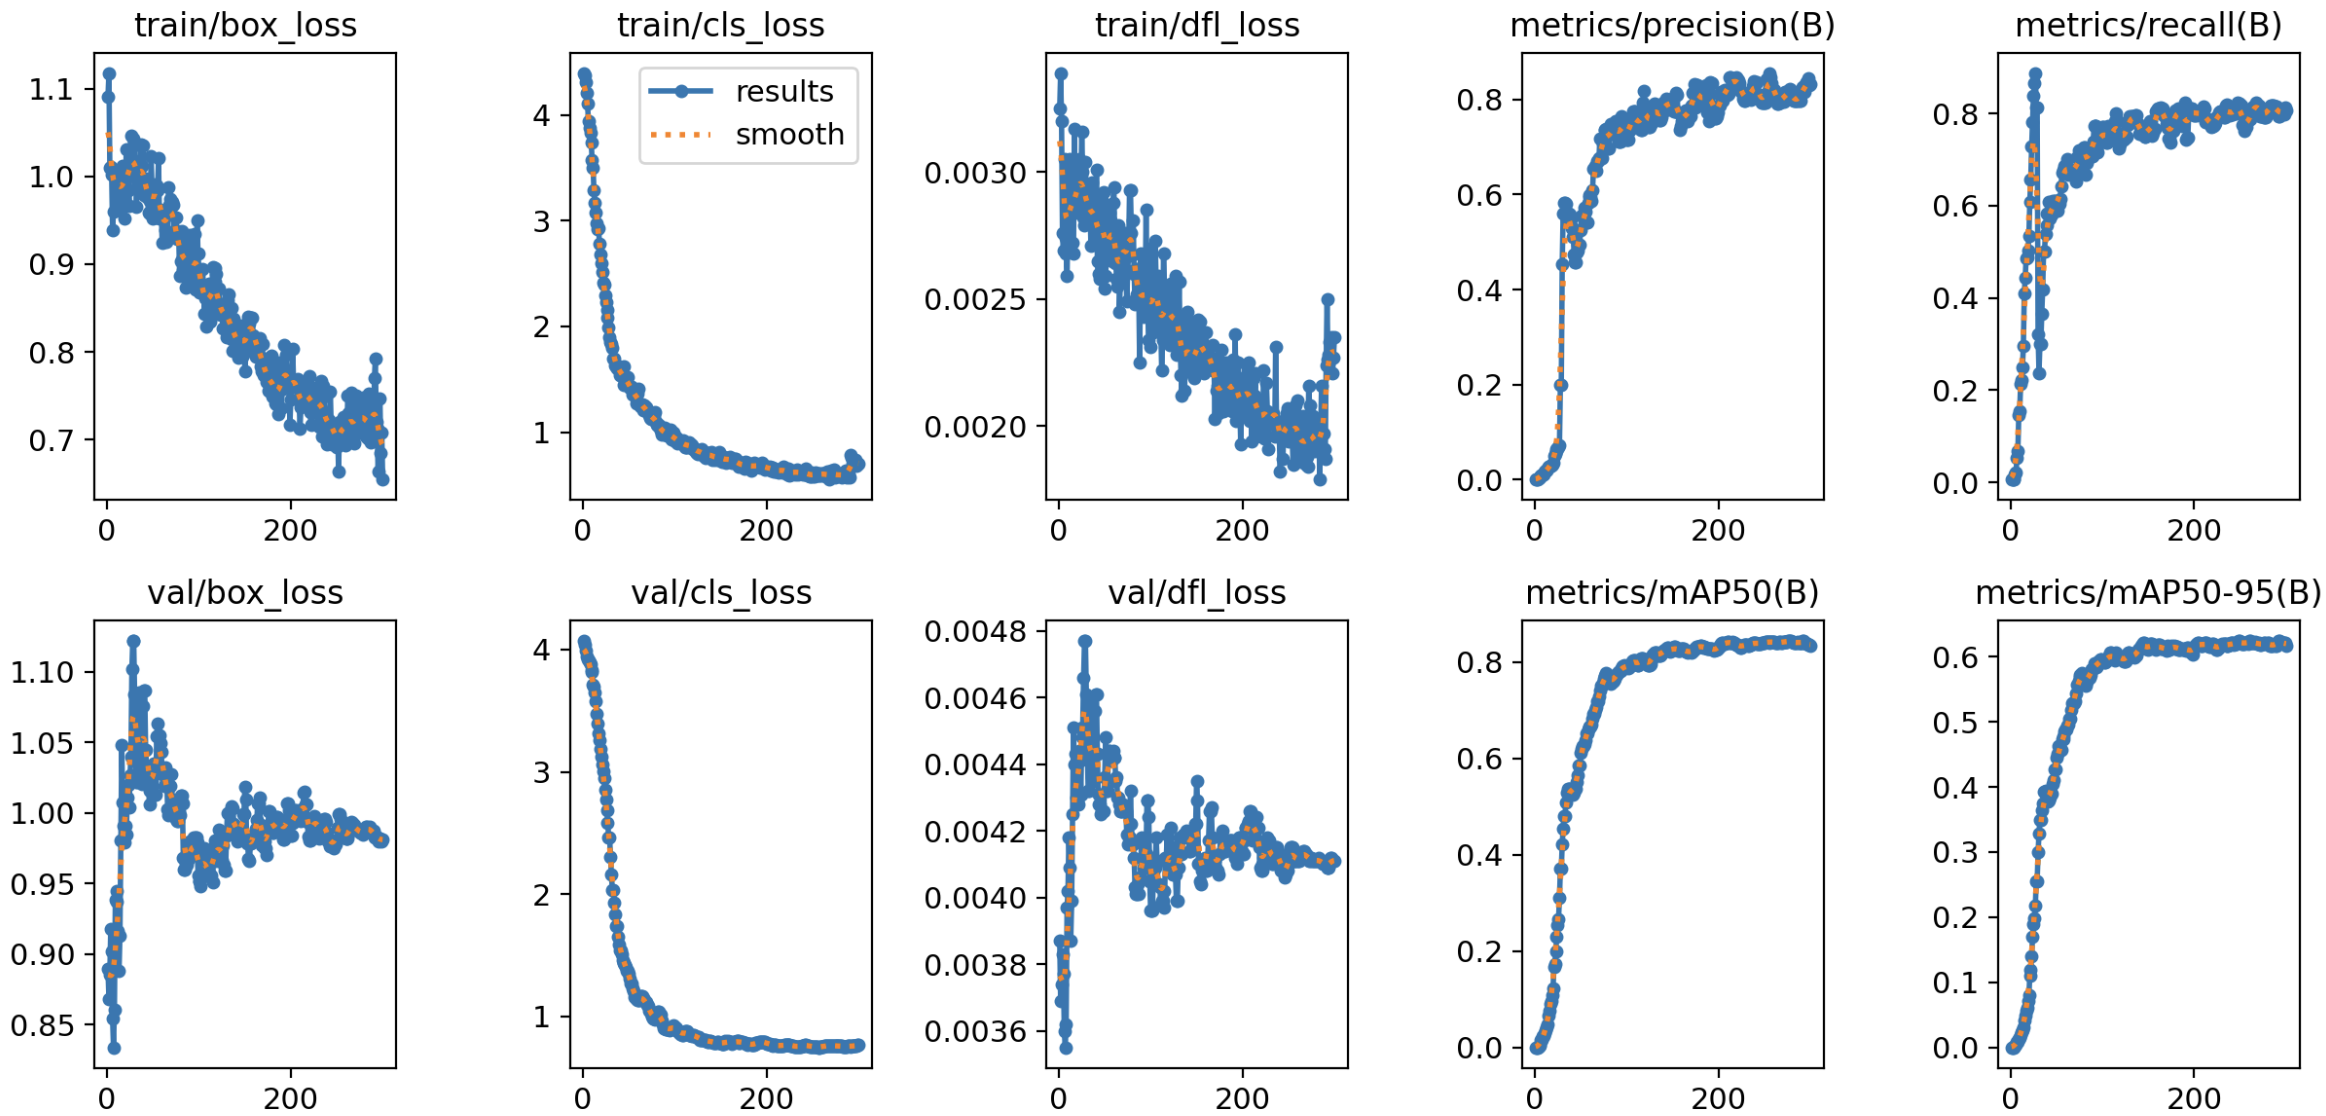
\includegraphics[width=1.01\linewidth]{latex/figures/Screenshot 2026-06-11 at 12.03.07.png}
    \caption[]{Plots of training results per epoch}
    \label{fig_trainingdatasetplots}
    \end{figure}

    \syncallcounters
    The normalized confusion matrix shows how well classes are recognized by the model. As shown in the figure shown below, most classes are classified correctly, as indicated by the strong diagonal values. However, light-grey objects were among the least correctly identified objects, this is a result of exposure and lighting changing enough to where the model will classify them as background. Some of objects were missed as background, a small amount of objects were misclassified, and some objects like dark-grey and white where confused with light-grey.
    \switchcolumn
    \begin{figure}[!htbp]
    \centering
    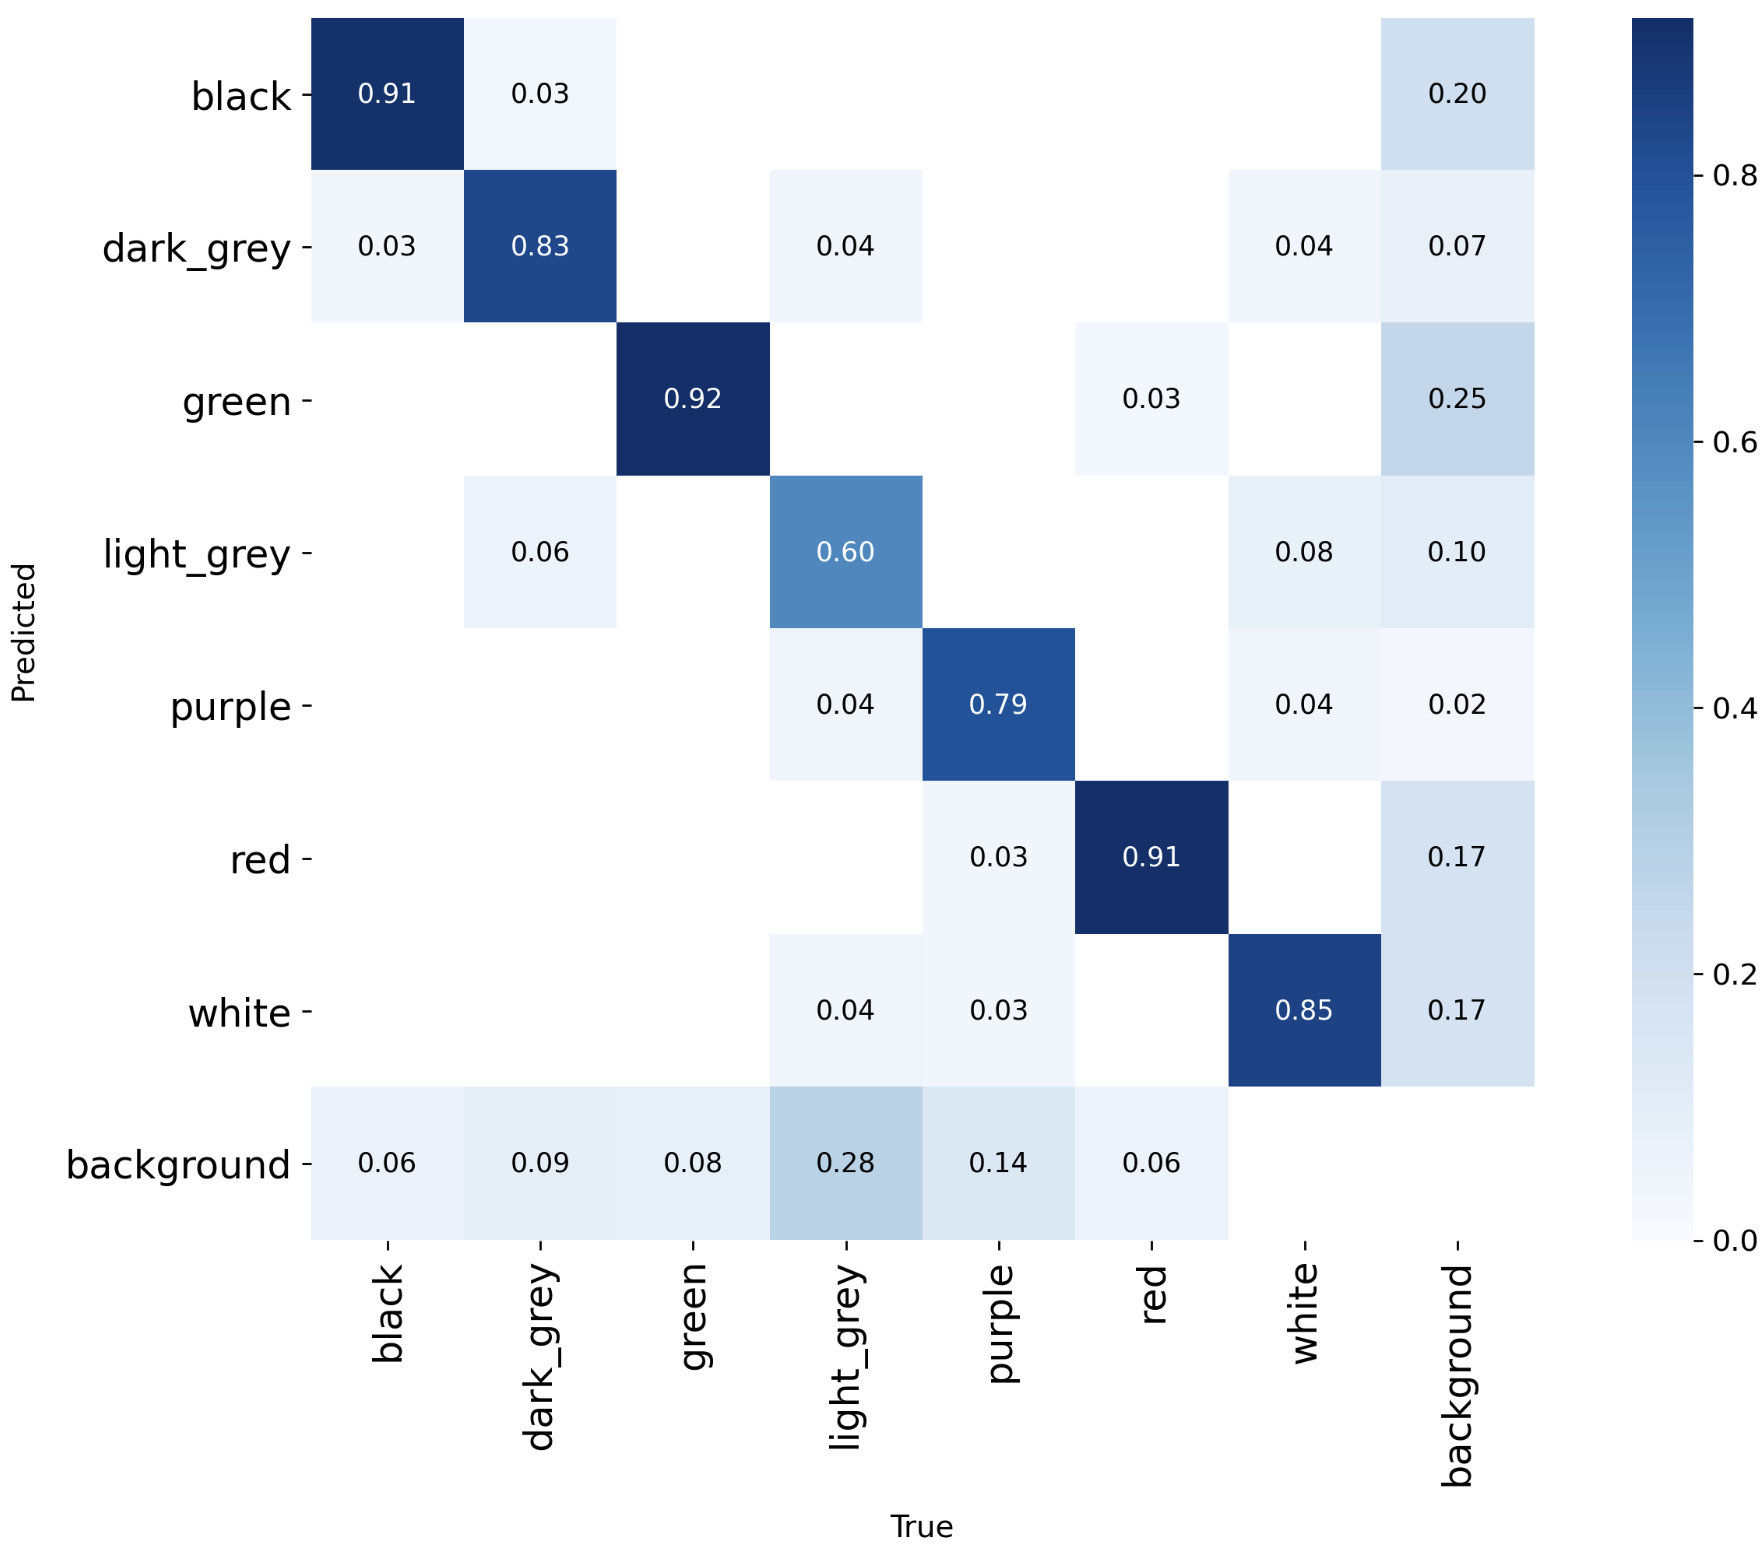
\includegraphics[width=1.01\linewidth]{latex/figures/Screenshot 2026-06-11 at 12.03.55.png}
    \caption[]{Normalised confusion matrix}
    \label{fig_trainingdatasetplots}
    \end{figure}
    \syncallcounters
    \centerline{\rule{7.8cm}{0.4pt}}
    A figure of the F1 confidence curve is shown below. This curve shows how the F1 metric, which combines precision (how many objects where correctly predicted) and recall (how many objects where correctly found), changes with the confidence threshold of the model. The curve shows that a good starting confidence threshold would be 0.3-0.35.
    \begin{figure}[!htbp]
    \centering
    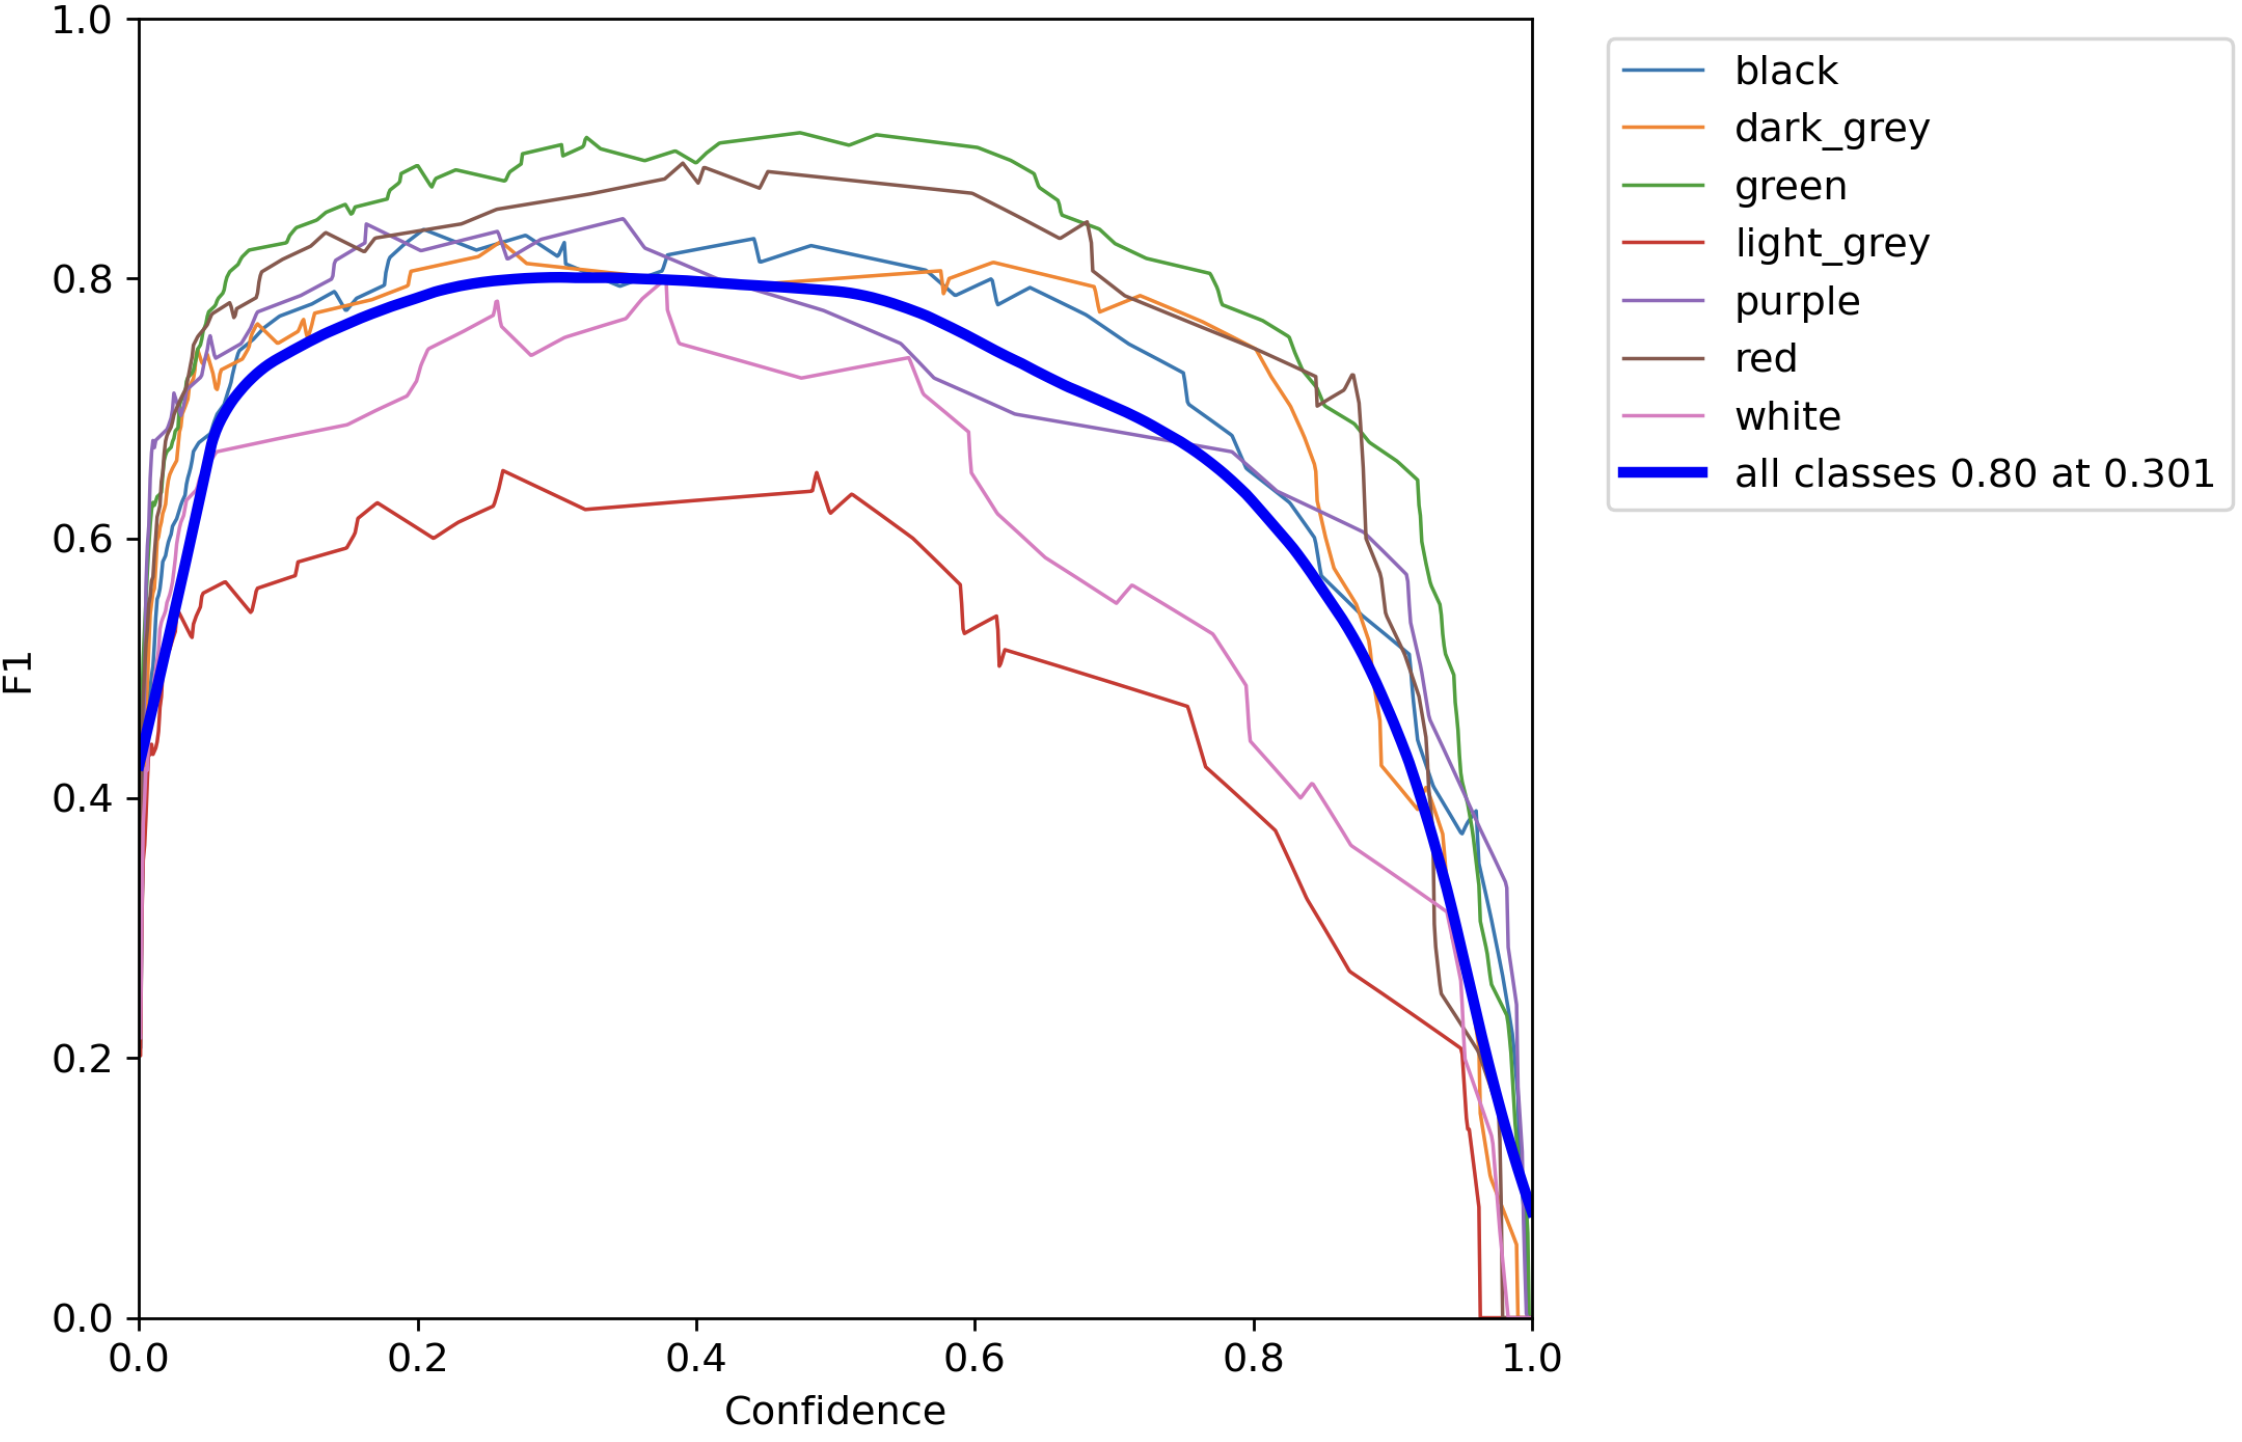
\includegraphics[width=1.02\linewidth]{latex/figures/Screenshot 2026-06-11 at 12.05.07.png}
    \caption[]{BoxF1 curve}
    \label{fig_trainingdatasetplots}
    \end{figure}
    
    \end{paracol}
    \newpage
    \subsubsection{Perception 3D}
    \begin{paracol}
        {2}
    \paragraph{Point Cloud-based Object localisation:}

    To determine the exact location of graspable objects around the MIRTE Master, the data gathered and transmitted by the camera must be interpreted. One effective method for achieving this is through the use of point clouds.
    
    As the name suggests, point clouds are collections of points that represent a three-dimensional space. These points may contain a variety of information, but the most important characteristic of a point during this project is its position, represented by its \textit{x}, \textit{y}, and \textit{z} coordinates. During this project, the \texttt{Open3D} library was used to process the point cloud. This particular library has been selected because of its user-friendly API and popularity over PCL \citep{zhou2018open3d}.
    
    Detecting planes will be done using the Random Sample Consensus model, or RANSAC for short. This algorithm picks a number of points from the point cloud at random and fits a plane through them. It then evaluates which points in the point cloud are within the given distance from the plane \citep{Randomsampleconsensus}. With this method, point clouds can easily and quickly be filtered such that only the important parts, namely the clusters of points representing small objects on the ground, remain.
    
    Next, an algorithm for discovering clusters is used called DBSCAN (Density-Based Spatial Clustering of Applications with Noise). The model evaluates the remaining points in the point cloud and determines the cluster to which they belong \citep{DBSCAN}. Afterwards, the identified clusters can be converted into bounding boxes, deciding an object's position and orientation, as well as its dimensions.
    \syncallcounters
    \switchcolumn
    Below, figures Figure~\ref{og_pc__} and Figure~\ref{bounding_boxes__} show the input to output the constructed point cloud pipeline.
    
     \begin{figure}[!htbp]
     \centering
     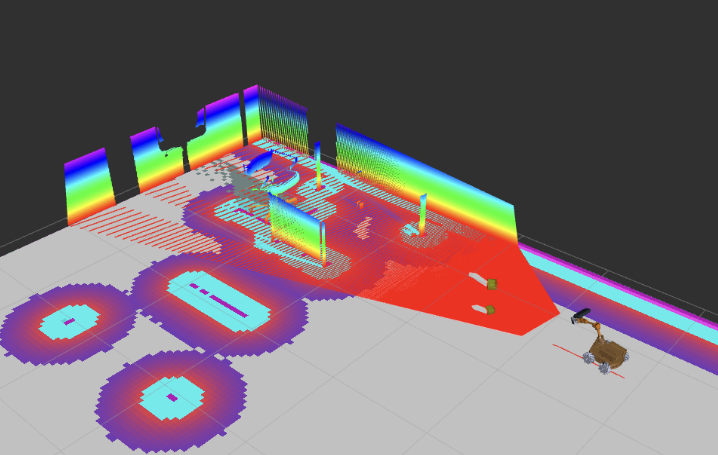
\includegraphics[width=0.99\linewidth]{latex/figures/Screenshot 2026-06-12 at 10.46.43.png}
     \caption[]{The point cloud as received from the camera topic}
     \label{og_pc__}
     \end{figure}
    
     \begin{figure}[!htbp]
     \centering
     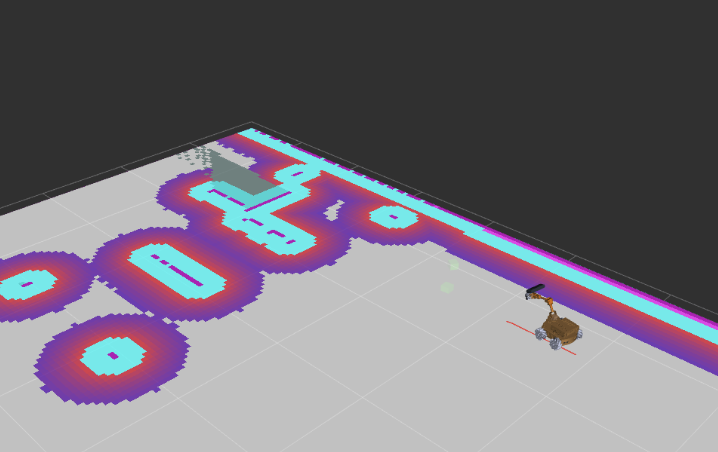
\includegraphics[width=0.99\linewidth]{latex/figures/Screenshot 2026-06-12 at 10.47.43.png}
     \caption[]{The resulting bounding boxes}
     \label{bounding_boxes__}
     \end{figure}
    
     Any objects that are in the costmap are excluded, resulting in only these bounding boxes remaining.

    %To determine the exact location of graspable objects around the MIRTE Master, the data gathered and sent by the camera will have to be interpreted in some way. One way to do so is using point clouds. These are, as the name suggests, clouds of points representing a 3-dimensional space. Points in these clouds can possess a variety of information, depending on their creator. However, the most important characteristic is a point's position, represented by \textit{x-}, \textit{y-}, and \textit{z-}coordinate values. This can be used to determine whether the point is part of a plane, e.g. the floor or a wall, but also desktops or table legs.

    %Detecting planes will be done using the Random Sample Consensus model, or RANSAC for short. This algorithm picks a number of points from the point cloud at random and fits a plane through them. It then evaluates which points in the point cloud are within the given distance from the plane \color{red}(Cite: Random Sample Consensus: A Paradigm for Model Fitting with Applications to Image Analysis and Automated Cartography)\color{black}. With this method, point clouds can easily and quickly be filtered such that only the important parts - the clusters of points representing small objects on the ground - remain.

    %Next, an algorithm for discovering clusters is used called DBSCAN (Density-Based Spatial Clustering of Applications with Noise). The model evaluates the remaining points in the point cloud and determines the cluster to which they belong \color{red}(cite A Density-Based Algorithm for Discovering Clusters in Large Spatial Databases with Noise)\color{black}. Afterwards, the identified clusters can be converted into bounding boxes, deciding an object's position and orientation, as well as its size. Finally, the poses (position \& orientation) of the localised objects are published to a ROS 2 topic, to be read by another node.
    \end{paracol}